%!TEX root = paper_ecg_cs_codec.tex
\section{Experiments and Discussion}
\label{sec:results}
The experiments in this section have been
designed to study the compression efficiency
of the encoder and the quality of reconstruction
under different reconstruction algorithms.


\begin{figure*}[ht]
\centering
\subfloat[$q$ vs $\prd$]{%
\includegraphics[width=0.32\linewidth]{images/rec_100_q_vs_prd_at_mr.pdf}}
\hfill
\subfloat[$q$ vs $\pss$]{%
\includegraphics[width=0.32\linewidth]{images/rec_100_q_vs_pss_at_mr.pdf}}
\hfill
\subfloat[$\pms$ vs $\pss$]{%
\includegraphics[width=0.32\linewidth]{images/rec_100_pms_vs_pss_at_q.pdf}}
\hfill
\caption{Variation of compression statistics vs quantization parameter
at different measurement ratios $\frac{m}{n}$
for record 100}
\label{fig-cs-codec-100-q-mr-stats}
\end{figure*}


\subsection{Quantization Parameter}
The quantization step is a key contributor to compression
savings. This can be studied better under the fixed
quantization mode. In the first experiment, we compress
the data from record 100 at different values of
the quantization parameter $q$ and PMS.
The results are shown in \cref{fig-cs-codec-100-q-mr-stats}.
The number of measurements ($m$) has been chosen to vary from
$20\%$ to $60\%$ of the window size ($n$).
$q$ varies from $0$ to $7$.
(a) shows that reconstruction quality doesn't
change much from $q=0$ till $q=4$ after which it starts degrading.
As expected, the PRD degrades as $m$ is reduced.
(b) shows that PSS (percentage space saving) increases linearly
with $q$. As $q$ increases, the size of the alphabet for
entropy coding reduces and this leads to increased space savings.
(c) shows the variation of PSS with PMS at different values of $q$.
PSS increases linearly with PMS. Also, PSS is much higher
than PMS at higher quantization levels.

Increasing quantization linearly increases the PSS.
Since up to $q=4$, there is no noticeable
impact on PRD, as seen in panel (a), it is safe
to enjoy these savings in bit rate. 
At $40\%$ PMS, one can attain up to $69.3\%$ PSS without
losing any reconstruction quality.

In the remaining experiments, we will be using adaptive
quantization.

\subsection{Compression across different records}

This additional space savings is the contribution
due to adaptive quantization and entropy coding.
The PRD is $5.6 \pm 1.8 \%$.
The quality score is $57.8 \pm 18.6$.
Quantization SNR is $37.3 \pm 0.9$ dB.
Our adaptive quantization algorithm ensures that the
quantization SNR doesn't vary much.


\subsection{Space Savings}

In this experiment, we report the variation of
the percentage space savings ($\pss$)
with the percentage measurement savings ($\pms$)
under different encoder configurations.
We chose the window size $n=512$.
PMS varies from $20\%$ to $80\%$.
Correspondingly $m$ varies from $410$ down to $77$.
For each choice of $m$ and $n$, we constructed
binary sensing matrices $\Phi$
for two different values of $d$ at $d=4$ and $d=12$.
All 48 records were encoded and $\pss$ was measured
separately for each of them.
\Cref{fig:res:pms-pss-errorbar} shows the variation
of mean $\pss$ (over records) with $\pms$ along with
error bars for standard deviation across records
at each $\pms$.
We note that $d=12$ gives slightly better compression.
However, the difference is not significant and it decreases
as PMS increases. The small error bars indicate that the
compression ratio doesn't vary much from record to record.
At low PMS, we can see that the compression scheme can
give additional savings of up to 25\%. The trend line
is linear and savings reduce linearly to 5\% at 85\% PMS.

\begin{figure}[!t]
\centering
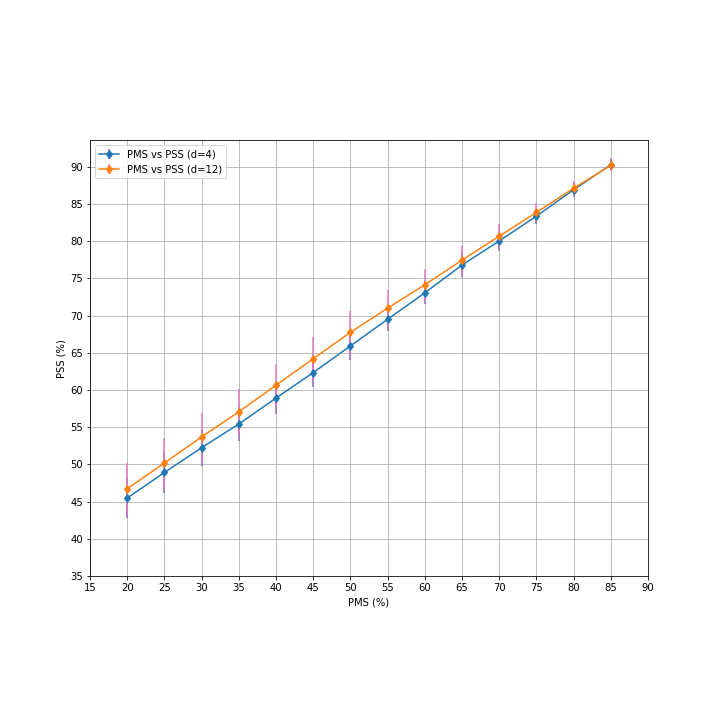
\includegraphics[width=0.95\linewidth]{images/bsbl/pms-vs-pss-errorbar.png}
\caption{Error bars for variation of mean $\pss$
with $\pms$ for 48 records at $d=4$ and $d=12$.}
\label{fig:res:pms-pss-errorbar}
\end{figure}

\Cref{fig:res:pms-pss-boxplot-d4} shows more detailed box plots
of variation of PMS across the 48 records at different PMS values.

\begin{figure}[!t]
\centering
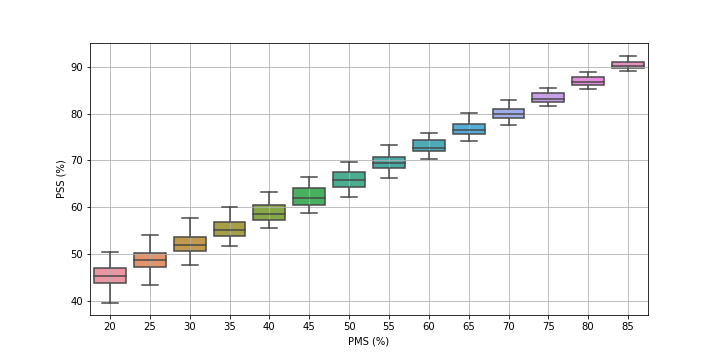
\includegraphics[width=0.95\linewidth]{images/bsbl/pms-vs-pss-boxplot-d4.png}
\caption{PMS vs PSS box plots over 48 records at $d=4$}
\label{fig:res:pms-pss-boxplot-d4}
\end{figure}
In the following, we will report results for $d=4$
configuration. Results are similar for $d=12$.

We measured the overhead of bits required to
encode the stream and frame headers. The overhead
varies from 0.07\% at PMS=20\% to about 0.4\% at PMS=80\%
on average. At higher PMS there are very few measurements
to encode. Hence overhead is higher. Increasing the frame
size will reduce the overhead. However, this will cause
delays in a real-time system since a frame cannot be decoded
till its full payload has been received. 

The bits per sample vary from
$6 \pm 0.3$ $\bps$ at PMS=20\% down to
$1 \pm 0.1$ $\bps$ at PMS=85\%.
This is significant compared to the uncompressed
rate of $11$ bits per sample.

Our adaptive quantization scheme is designed to
keep the noise introduced by quantization and clipping
steps to reasonable levels.
\Cref{fig:res:pms-q-snr-boxplot-d4} shows the box plots
of variation of quantization noise SNR across the 48
records at different PMS. It is clear that quantization
SNR remains limited between 35 and 40 dB.

\begin{figure}[!t]
\centering
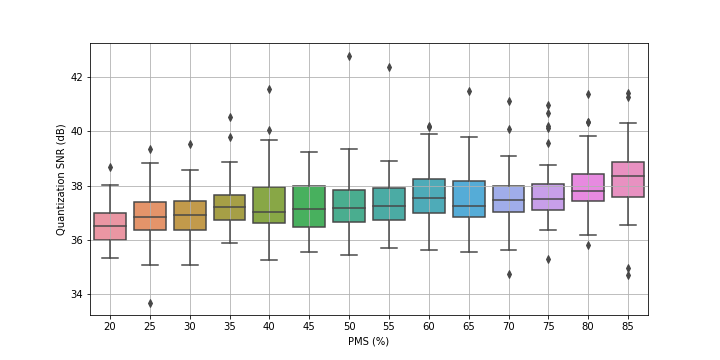
\includegraphics[width=0.95\linewidth]{images/bsbl/pms-vs-q-snr-boxplot-d4.png}
\caption{PMS vs Quantization SNR box plots over 48 records at $d=4$}
\label{fig:res:pms-q-snr-boxplot-d4}
\end{figure}

\subsection{Reconstruction with BSBL-BO}

\begin{figure}[!t]
\centering
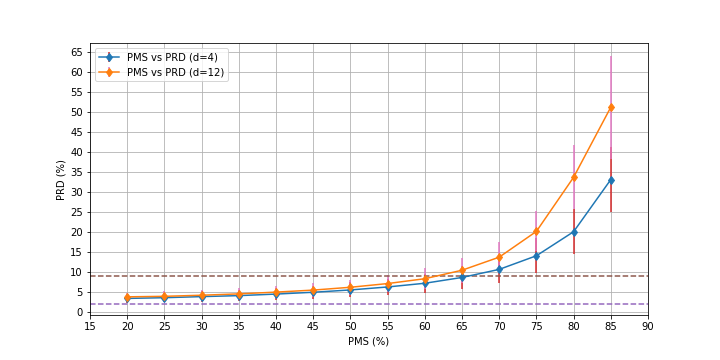
\includegraphics[width=0.95\linewidth]{images/bsbl/pms-vs-prd-errorbar.png}
\caption{Error bars for variation of PMS vs mean PRD at $d=4$ and $d=12$ for reconstruction with BSBL-BO algorithm.}
\label{fig:res:bsbl-pms-prd-errorbar}
\end{figure}


\begin{figure}[!t]
\centering
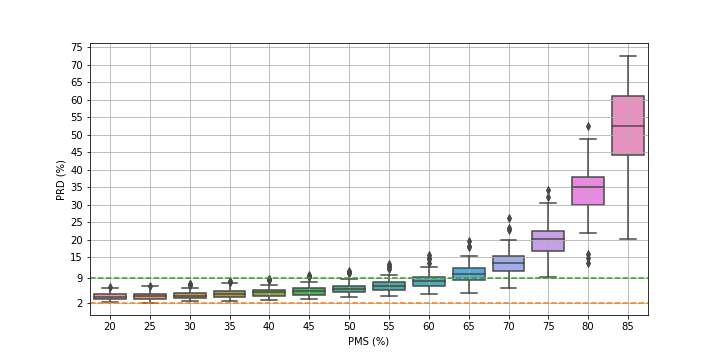
\includegraphics[width=0.95\linewidth]{images/bsbl/pms-vs-prd-boxplot-d12.png}
\caption{PMS vs PRD box plots over 48 records at $d=12$ for reconstruction
with BSBL-BO algorithm.}
\label{fig:res:bsbl-pms-prd-boxplot-d12}
\end{figure}

\begin{figure}[!t]
\centering
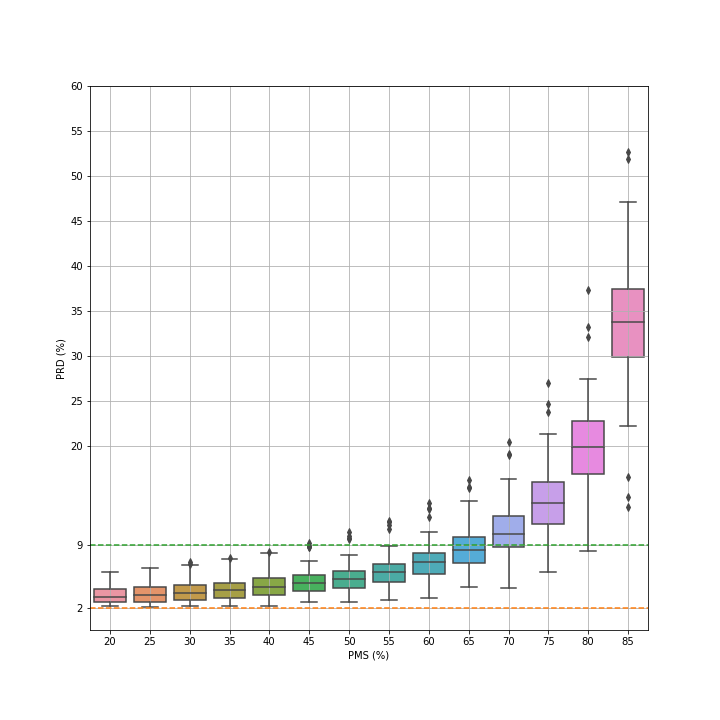
\includegraphics[width=0.95\linewidth]{images/bsbl/pms-vs-prd-boxplot-d4.png}
\caption{PMS vs PRD box plots over 48 records at $d=4$ for reconstruction
with BSBL-BO algorithm}
\label{fig:res:bsbl-pms-prd-boxplot-d4}
\end{figure}

\subsection{Reconstruction with CS-NET}


\begin{figure}[!t]
\centering
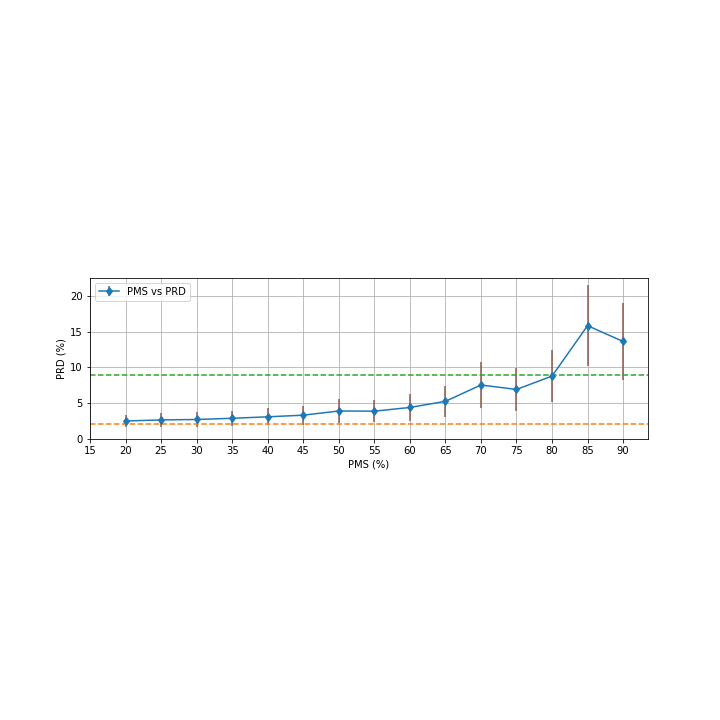
\includegraphics[width=0.95\linewidth]{images/csnet/pms-vs-prd-errorbar.png}
\caption{Error bars for variation of PMS vs mean PRD at $d=4$ for reconstruction with
CS-NET.}
\label{fig:res:csnet-pms-prd-errorbar}
\end{figure}

\begin{figure}[!t]
\centering
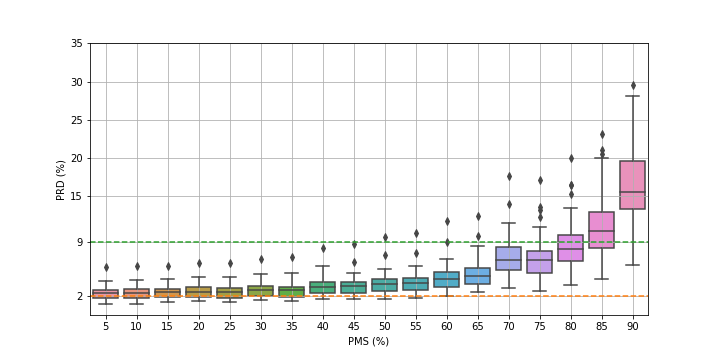
\includegraphics[width=0.95\linewidth]{images/csnet/pms-vs-prd-boxplot.png}
\caption{PMS vs PRD box plots over 48 records at $d=4$ for reconstruction
with CS-NET}
\label{fig:res:csnet-pms-prd-boxplot}
\end{figure}
